\documentclass[11pt]{article}
\usepackage[margin=0.8in]{geometry}
\usepackage{booktabs}
\usepackage{graphicx}
\usepackage{float}
\usepackage{longtable}
\title{Presentation Results Pack: LoRA Geometry + Oracle Routing}
\author{}
\date{}

\begin{document}
\maketitle

\section*{Experiment Overview}
\begin{tabular}{p{0.28\linewidth}p{0.67\linewidth}}
\toprule
Experiment & Key measured result \\
\midrule
Exp 1: Full-FT SVD (SST-2 q/v) & Mean cumulative energy at k=64 is 0.7068; k=107 reaches 80\% energy. \\
Exp 2: LoRA-FT subspace overlap (SST-2 q/v) & Mean overlap rises from 0.0472 at k=1 to 0.1228 at k=64 (computed over 24 matrices). \\
Exp 3: Oracle-routed LoRA experts across 6 GLUE tasks & Weighted primary = 0.8919; vs per-task Full-FT weighted primary delta = -0.0018; end-to-end runtime = 44.61s. \\
\bottomrule
\end{tabular}


\section*{Experiment 1: Full-FT Spectral Energy (SST-2)}
\begin{figure}[H]
\centering
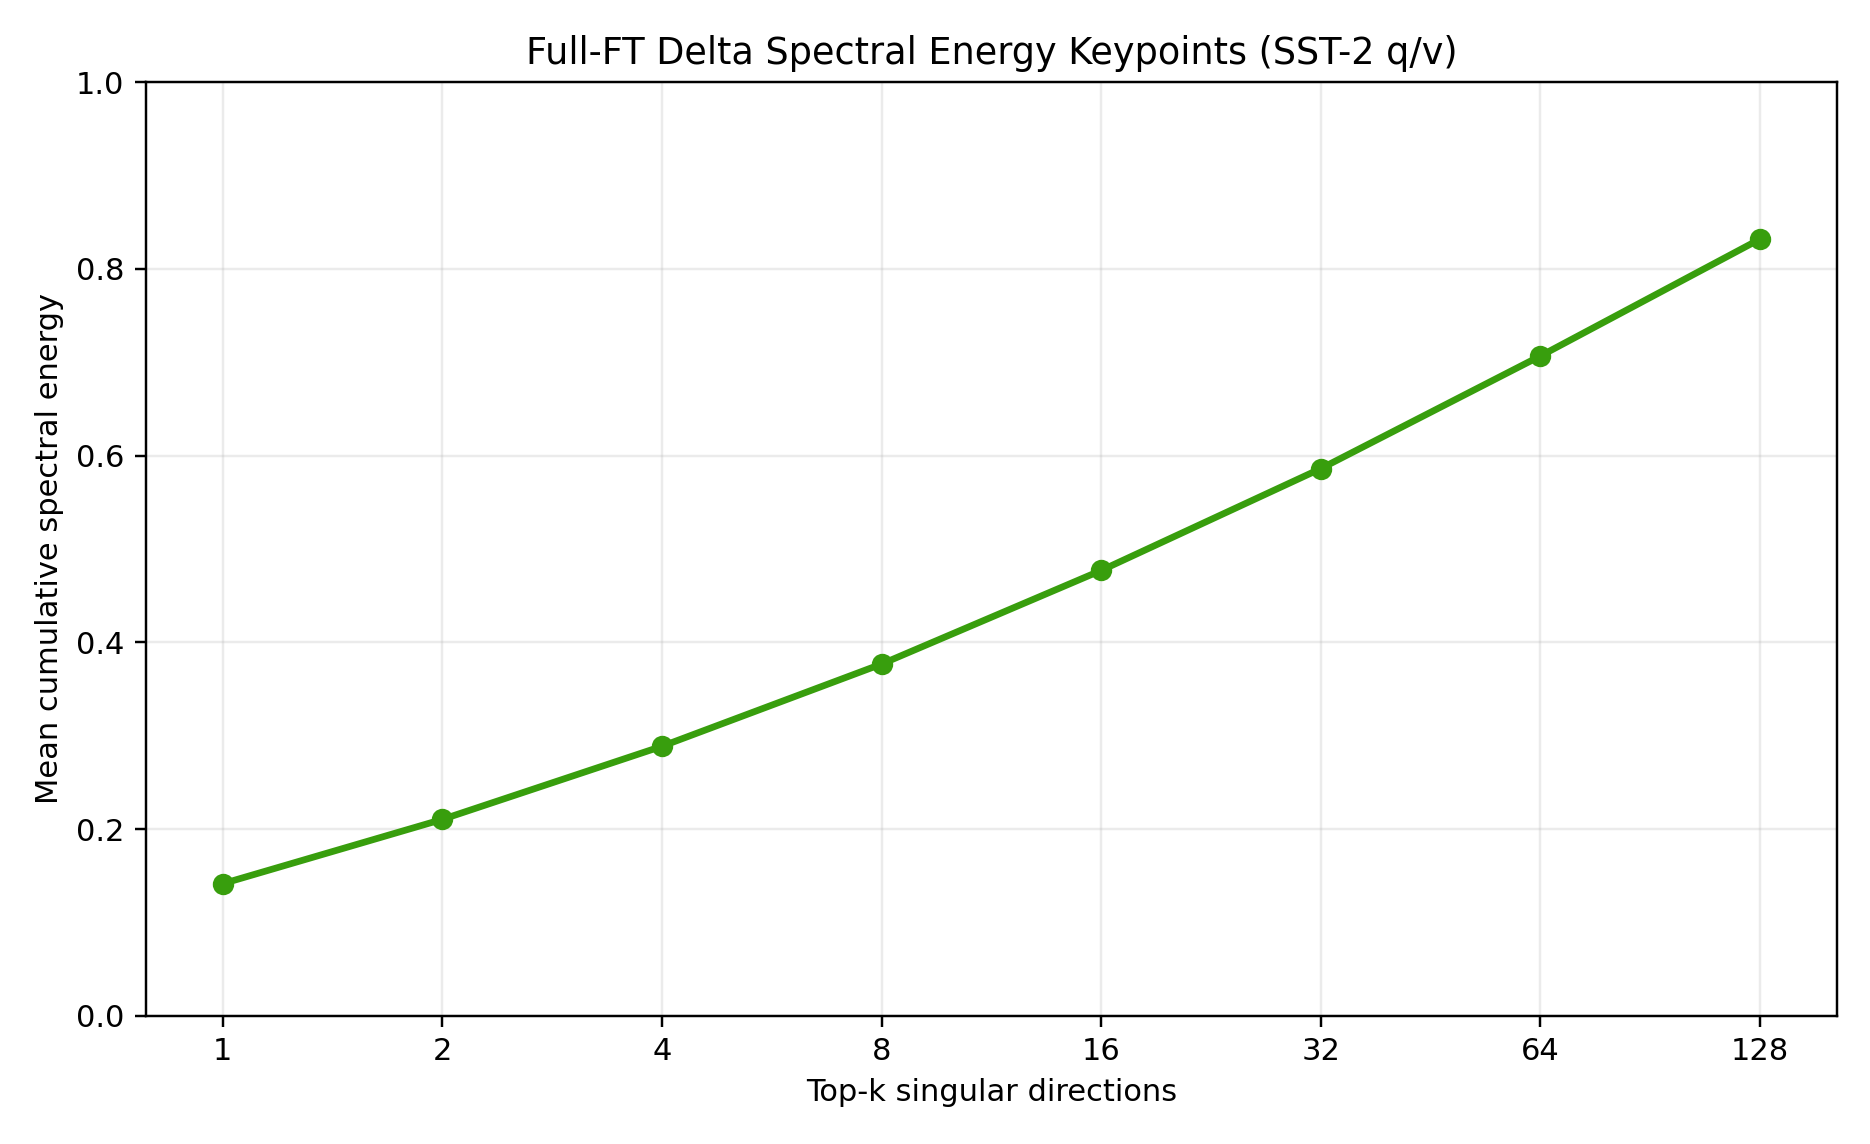
\includegraphics[width=0.85\linewidth]{figures/svd_energy_keypoints.png}
\caption{Mean cumulative spectral energy across SST-2 query/value update matrices.}
\end{figure}
\begin{tabular}{rr}
\toprule
k & Mean cumulative energy \\
\midrule
1 & 0.1415 \\
2 & 0.2104 \\
4 & 0.2887 \\
8 & 0.3768 \\
16 & 0.4770 \\
32 & 0.5861 \\
64 & 0.7068 \\
128 & 0.8320 \\
\midrule
$k$ for 80\% energy & 107 \\
$k$ for 90\% energy & 128 \\
$k$ for 95\% energy & 128 \\
\bottomrule
\end{tabular}


\section*{Experiment 2: LoRA vs Full-FT Subspace Overlap (SST-2)}
\begin{figure}[H]
\centering
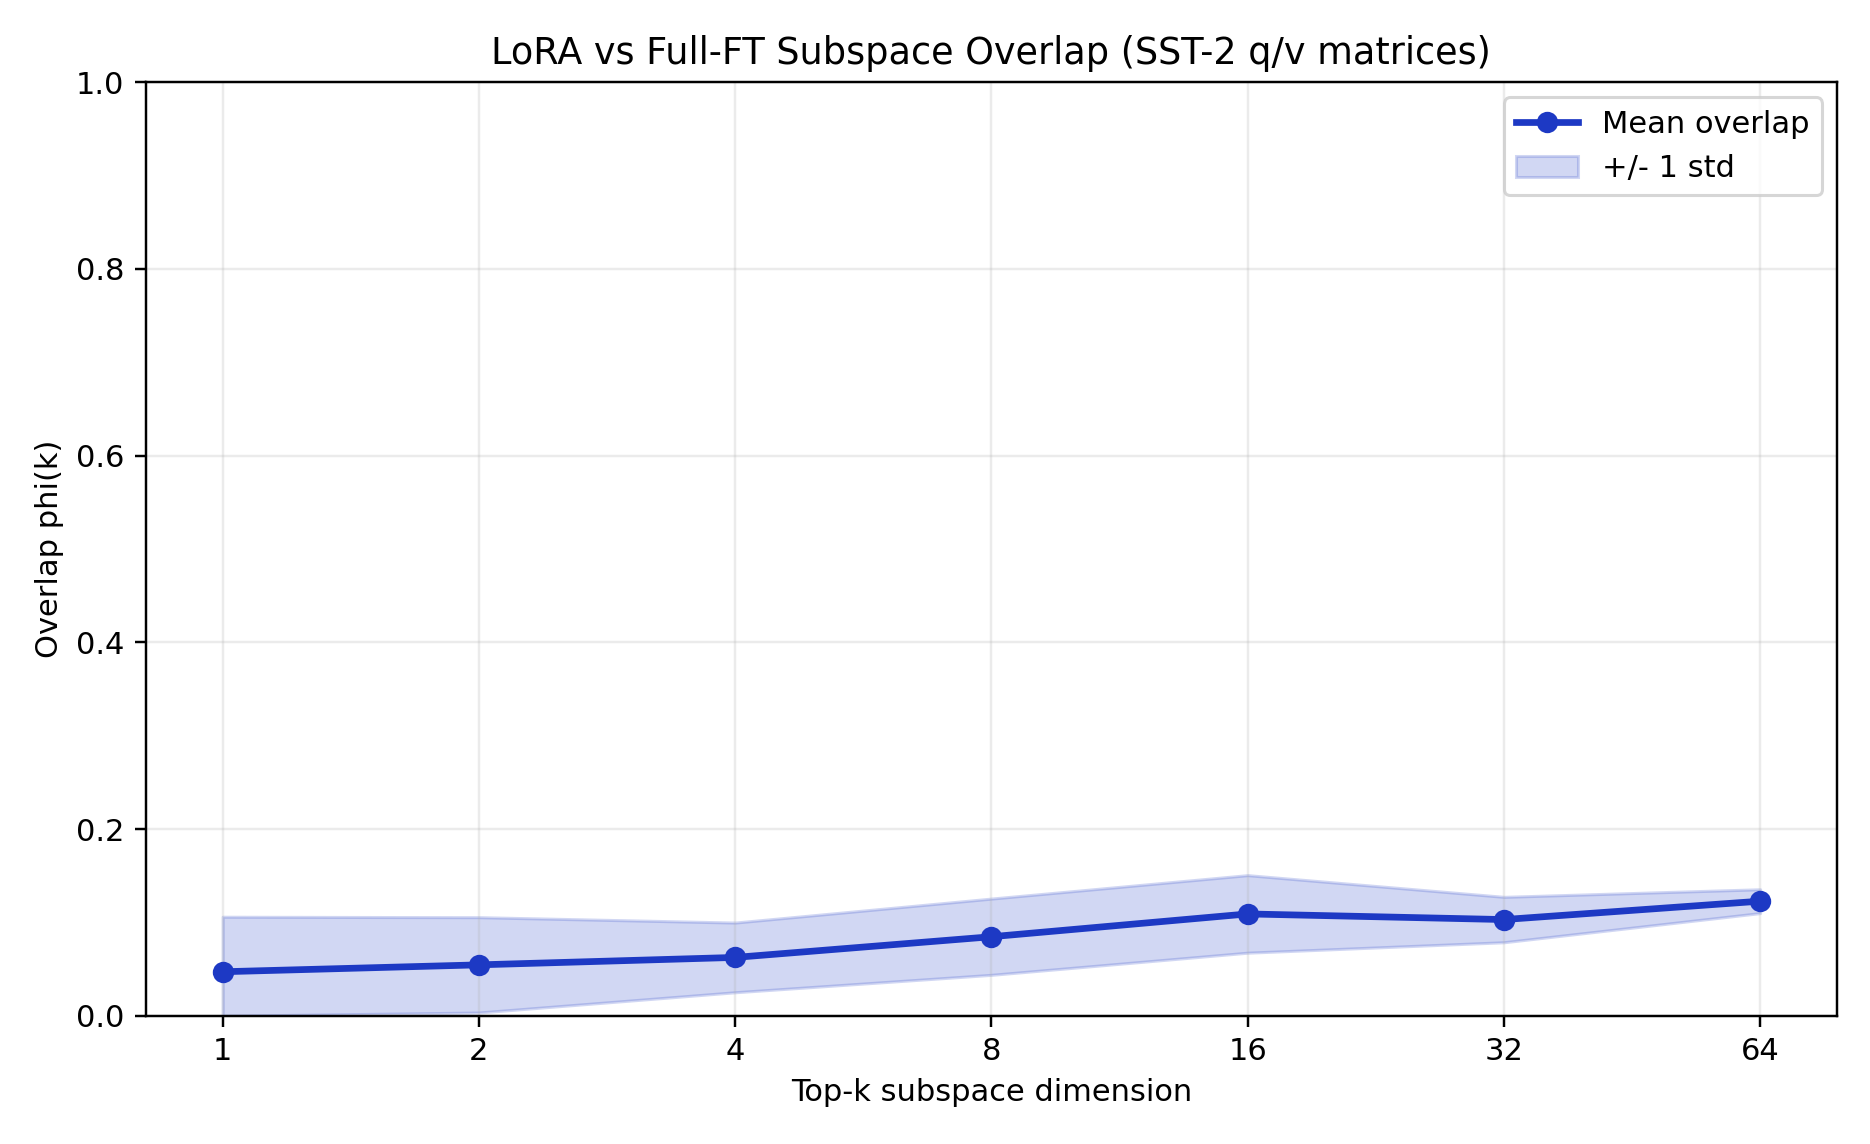
\includegraphics[width=0.85\linewidth]{figures/subspace_overlap_mean_std.png}
\caption{Subspace overlap $\phi(k)$ with mean and $\pm 1$ std across matrices.}
\end{figure}
\begin{tabular}{rrrrr}
\toprule
k & Mean overlap $\phi(k)$ & Std & Min & Max \\
\midrule
1 & 0.0472 & 0.0589 & 0.0000 & 0.2592 \\
2 & 0.0546 & 0.0510 & 0.0078 & 0.2029 \\
4 & 0.0625 & 0.0373 & 0.0162 & 0.1636 \\
8 & 0.0847 & 0.0408 & 0.0272 & 0.1933 \\
16 & 0.1091 & 0.0415 & 0.0500 & 0.1837 \\
32 & 0.1031 & 0.0243 & 0.0654 & 0.1454 \\
64 & 0.1228 & 0.0128 & 0.0987 & 0.1433 \\
\bottomrule
\end{tabular}


\section*{Experiment 3: Oracle-Routed LoRA vs Baselines (6 GLUE tasks)}
\begin{figure}[H]
\centering
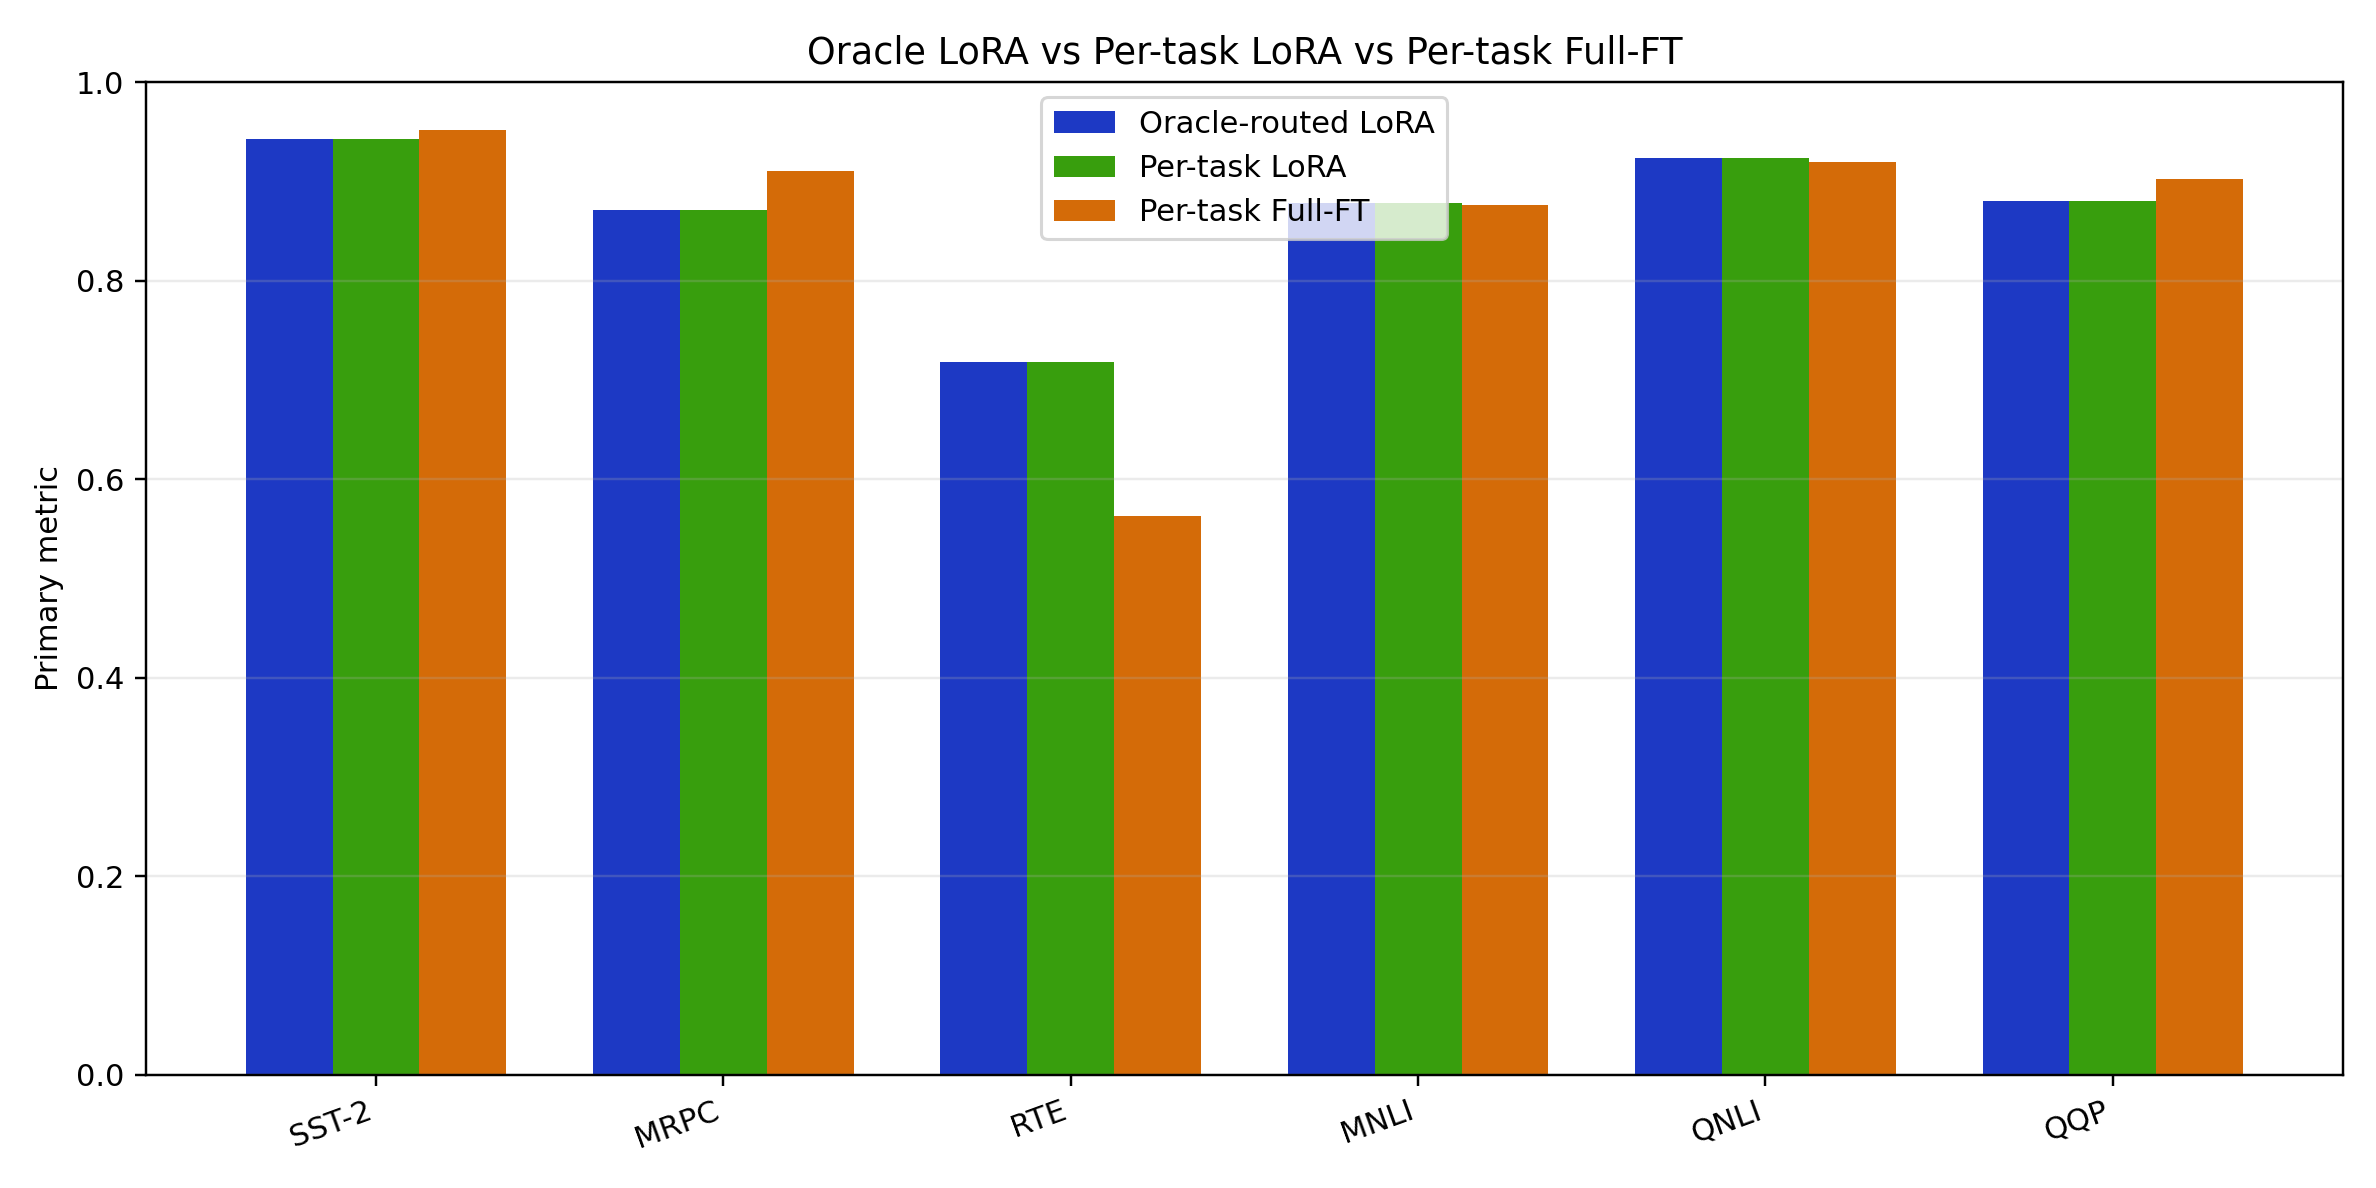
\includegraphics[width=0.90\linewidth]{figures/oracle_vs_baselines_per_task.png}
\caption{Primary metric comparison by task.}
\end{figure}

\begin{figure}[H]
\centering
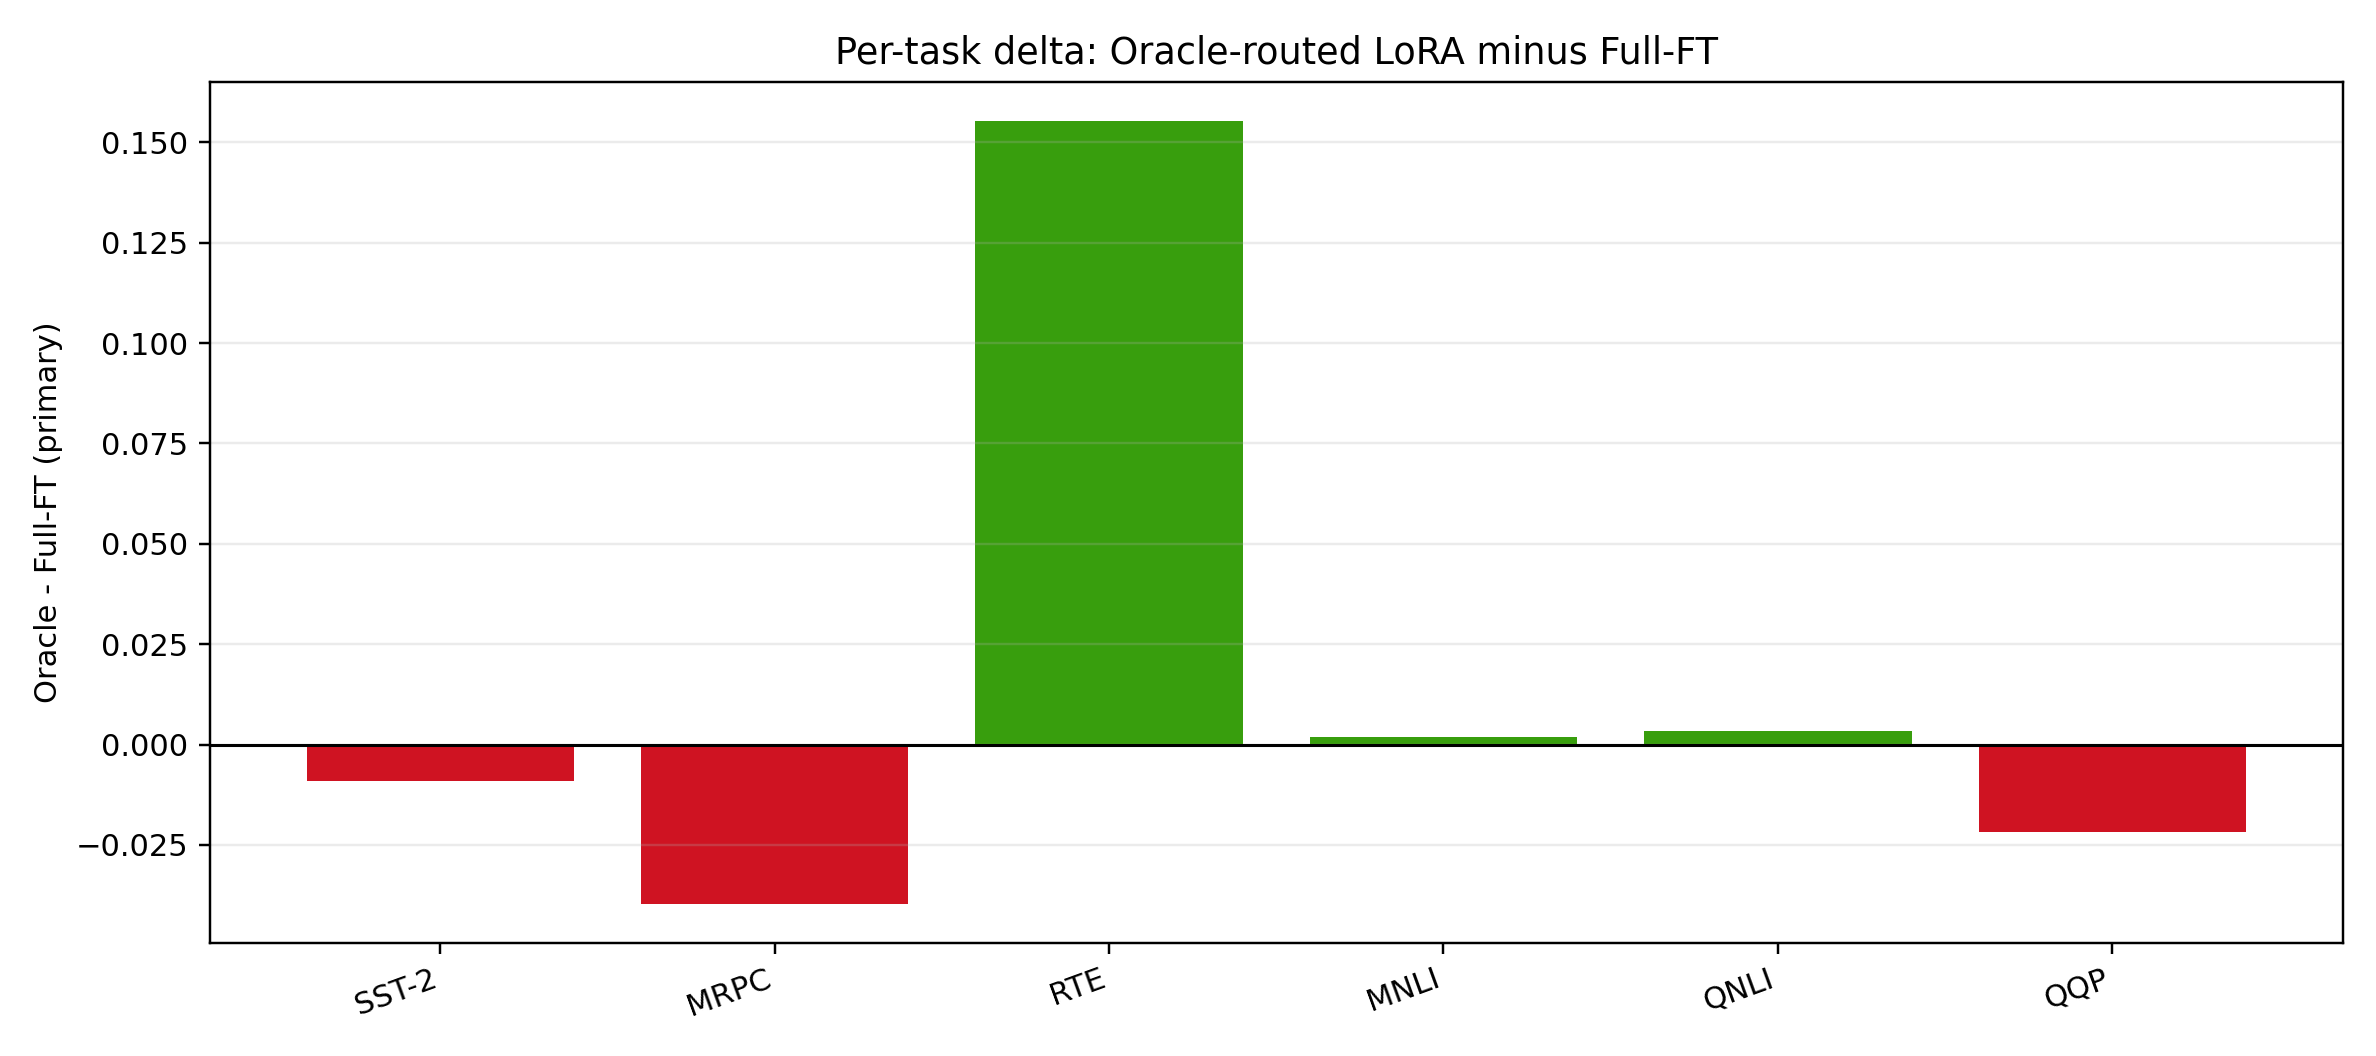
\includegraphics[width=0.90\linewidth]{figures/oracle_minus_fft_delta.png}
\caption{Per-task primary-metric delta between oracle-routed LoRA and per-task Full-FT.}
\end{figure}

\begin{tabular}{lrrrrrr}
\toprule
Task & N & Oracle & LoRA & Full-FT & Oracle-LoRA & Oracle-FT \\
\midrule
SST-2 & 872 & 0.9427 & 0.9427 & 0.9518 & 0.0000 & -0.0092 \\
MRPC & 408 & 0.8709 & 0.8709 & 0.9105 & 0.0000 & -0.0396 \\
RTE & 277 & 0.7184 & 0.7184 & 0.5632 & 0.0000 & 0.1552 \\
MNLI & 2000 & 0.8780 & 0.8780 & 0.8760 & 0.0000 & 0.0020 \\
QNLI & 2000 & 0.9235 & 0.9235 & 0.9200 & 0.0000 & 0.0035 \\
QQP & 2000 & 0.8804 & 0.8804 & 0.9021 & 0.0000 & -0.0217 \\
\bottomrule
\end{tabular}


\vspace{0.5em}
\begin{tabular}{lrrrrr}
\toprule
Metric & Oracle & LoRA & Full-FT & Oracle-LoRA & Oracle-FT \\
\midrule
Macro primary & 0.8690 & 0.8690 & 0.8539 & 0.0000 & 0.0150 \\
Weighted primary & 0.8919 & 0.8919 & 0.8937 & 0.0000 & -0.0018 \\
Macro accuracy & 0.8690 & 0.8690 & 0.8545 & 0.0000 & 0.0145 \\
Weighted accuracy & 0.8963 & 0.8963 & 0.8974 & 0.0000 & -0.0012 \\
\bottomrule
\end{tabular}


\end{document}
